\begin{flushright} {\tiny {\color{gray} basis\_q2\_3D.tex}} \end{flushright}
%~~~~~~~~~~~~~~~~~~~~~~~~~~~~~~~~~~~~~~~~~~~~~~~~~~~~~~~~~~~~~~~~~~~~~~~~~~~~~~~~~~~~~~~~~~~~~~~~~~

\begin{center}
\begin{flushright} {\tiny {\color{gray} (tikz\_q2.tex)}} \end{flushright}
%~~~~~~~~~~~~~~~~~~~~~~~~~~~~~~~~~~~~~~~~~~~~~~~~~~~~~~~~~~~~~~~~~~~~~~~~~~~~~~~~~~~~~~~~~~~~~~~~~~

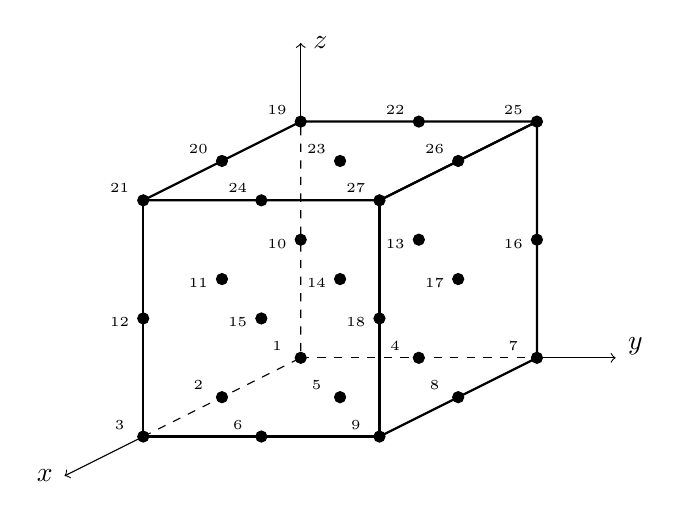
\begin{tikzpicture}
%\draw[fill=gray!23,gray!23](0,0) rectangle (9,7);
%\draw[step=0.5cm,gray,very thin] (0,0) grid (9,7); %background grid

\draw[thick] (2,4.5) -- (5,4.5) -- (7,5.5) -- (4,5.5) -- cycle; %top
\draw[thick] (2,1.5) -- (5,1.5) -- (5,4.5) -- (2,4.5) -- cycle; %front
\draw[thick] (5,1.5) -- (7,2.5) -- (7,5.5) -- (5,4.5) -- cycle; %right

\draw[dashed]   (2,1.5) -- (4,2.5) -- (4,5.5) ; % 
\draw[dashed]   (4,2.5) -- (7,2.5)  ; % 

\draw[thin,->] (2,1.5) -- (1,1); %x
\draw[thin,->] (7,2.5) -- (8,2.5); %y
\draw[thin,->] (4,5.5) -- (4,6.5); %z
\node[] at (0.75,1) {$x$};
\node[] at (8.25,2.65) {$y$};
\node[] at (4.25,6.5) {$z$};

\draw[black,fill=black] (4,2.5)   circle (2pt);
\draw[black,fill=black] (3,2)   circle (2pt);
\draw[black,fill=black] (2,1.5)   circle (2pt);
\draw[black,fill=black] (5.5,2.5)   circle (2pt);
\draw[black,fill=black] (4.5,2)   circle (2pt);
\draw[black,fill=black] (3.5,1.5)   circle (2pt);
\draw[black,fill=black] (7,2.5)   circle (2pt);
\draw[black,fill=black] (6,2)   circle (2pt);
\draw[black,fill=black] (5,1.5)   circle (2pt);

\draw[black,fill=black] (4,4)   circle (2pt);
\draw[black,fill=black] (3,3.5)   circle (2pt);
\draw[black,fill=black] (2,3)   circle (2pt);
\draw[black,fill=black] (5.5,4)   circle (2pt);
\draw[black,fill=black] (4.5,3.5)   circle (2pt);
\draw[black,fill=black] (3.5,3)   circle (2pt);
\draw[black,fill=black] (7,4)   circle (2pt);
\draw[black,fill=black] (6,3.5)   circle (2pt);
\draw[black,fill=black] (5,3)   circle (2pt);

\draw[black,fill=black] (4,5.5)   circle (2pt);
\draw[black,fill=black] (3,5)   circle (2pt);
\draw[black,fill=black] (2,4.5)   circle (2pt);
\draw[black,fill=black] (5.5,5.5)   circle (2pt);
\draw[black,fill=black] (4.5,5)   circle (2pt);
\draw[black,fill=black] (3.5,4.5)   circle (2pt);
\draw[black,fill=black] (7,5.5)   circle (2pt);
\draw[black,fill=black] (6,5)   circle (2pt);
\draw[black,fill=black] (5,4.5)   circle (2pt);

\node[] at (3.7,2.65) {\tiny 1};
\node[] at (2.7,2.15) {\tiny 2};
\node[] at (1.7,1.65) {\tiny 3};
\node[] at (5.2,2.65) {\tiny 4};
\node[] at (4.2,2.15) {\tiny 5};
\node[] at (3.2,1.65) {\tiny 6};
\node[] at (6.7,2.65) {\tiny 7};
\node[] at (5.7,2.15) {\tiny 8};
\node[] at (4.7,1.65) {\tiny 9};

\node[] at (3.7,3.95) {\tiny 10};
\node[] at (2.7,3.45) {\tiny 11};
\node[] at (1.7,2.95) {\tiny 12};
\node[] at (5.2,3.95) {\tiny 13};
\node[] at (4.2,3.45) {\tiny 14};
\node[] at (3.2,2.95) {\tiny 15};
\node[] at (6.7,3.95) {\tiny 16};
\node[] at (5.7,3.45) {\tiny 17};
\node[] at (4.7,2.95) {\tiny 18};

\node[] at (3.7,5.65) {\tiny 19};
\node[] at (2.7,5.15) {\tiny 20};
\node[] at (1.7,4.65) {\tiny 21};
\node[] at (5.2,5.65) {\tiny 22};
\node[] at (4.2,5.15) {\tiny 23};
\node[] at (3.2,4.65) {\tiny 24};
\node[] at (6.7,5.65) {\tiny 25};
\node[] at (5.7,5.15) {\tiny 26};
\node[] at (4.7,4.65) {\tiny 27};
\end{tikzpicture}


\end{center}

\begin{eqnarray}
\bN_{1} &=& 0.5r(r-1)  \cdot 0.5s(s-1) \cdot 0.5t(t-1) \nn\\
\bN_{2} &=& (1-r^2)    \cdot 0.5s(s-1) \cdot 0.5t(t-1) \nn\\
\bN_{3} &=& 0.5r(r+1)  \cdot 0.5s(s-1) \cdot 0.5t(t-1) \nn\\
\bN_{4} &=&  0.5r(r-1) \cdot (1-s^2)   \cdot 0.5t(t-1) \nn\\
\bN_{5} &=&  (1-r^2)   \cdot (1-s^2)   \cdot 0.5t(t-1) \nn\\
\bN_{6} &=& 0.5r(r+1)  \cdot (1-s^2)   \cdot 0.5t(t-1) \nn\\
\bN_{7} &=&  0.5r(r-1) \cdot 0.5s(s+1) \cdot 0.5t(t-1) \nn\\
\bN_{8} &=&  (1-r^2)   \cdot 0.5s(s+1) \cdot 0.5t(t-1) \nn\\
\bN_{9} &=& 0.5r(r+1)  \cdot 0.5s(s+1) \cdot 0.5t(t-1) \nn\\
\bN_{10}&=&  0.5r(r-1) \cdot 0.5s(s-1) \cdot (1-t^2) \nn\\
\bN_{11}&=&  (1-r^2)   \cdot 0.5s(s-1) \cdot (1-t^2) \nn\\
\bN_{12}&=& 0.5r(r+1)  \cdot 0.5s(s-1) \cdot (1-t^2) \nn\\
\bN_{13}&=&  0.5r(r-1) \cdot (1-s^2)   \cdot (1-t^2) \nn\\
\bN_{14}&=&  (1-r^2)   \cdot (1-s^2)   \cdot (1-t^2) \nn\\
\bN_{15}&=& 0.5r(r+1)  \cdot (1-s^2)   \cdot (1-t^2) \nn\\
\bN_{16}&=&  0.5r(r-1) \cdot 0.5s(s+1) \cdot (1-t^2) \nn\\
\bN_{17}&=&  (1-r^2)   \cdot 0.5s(s+1) \cdot (1-t^2) \nn\\
\bN_{18}&=& 0.5r(r+1)  \cdot 0.5s(s+1) \cdot (1-t^2) \nn\\
\bN_{19}&=&  0.5r(r-1) \cdot 0.5s(s-1) \cdot 0.5t(t+1) \nn\\
\bN_{20}&=&  (1-r^2)   \cdot 0.5s(s-1) \cdot 0.5t(t+1) \nn\\
\bN_{21}&=& 0.5r(r+1)  \cdot 0.5s(s-1) \cdot 0.5t(t+1) \nn\\
\bN_{22}&=&  0.5r(r-1) \cdot (1-s^2)   \cdot 0.5t(t+1) \nn\\
\bN_{23}&=&  (1-r^2)   \cdot (1-s^2)   \cdot 0.5t(t+1) \nn\\
\bN_{24}&=& 0.5r(r+1)  \cdot (1-s^2)   \cdot 0.5t(t+1) \nn\\
\bN_{25}&=&  0.5r(r-1) \cdot 0.5s(s+1) \cdot 0.5t(t+1) \nn\\
\bN_{26}&=&  (1-r^2)   \cdot 0.5s(s+1) \cdot 0.5t(t+1) \nn\\
\bN_{27}&=& 0.5r(r+1)  \cdot 0.5s(s+1) \cdot 0.5t(t+1) \nn
\end{eqnarray}






